%%%%%%%%%%%%%%%%%%%%%%%%%%%%%%%%%%%%%%%%%%%%%%%%%%%%%%%%%%%%%%%%
%  Template for creating scribe notes for MAT 308
%
%  Fill in your name, lecture number, lecture date and body
%  of scribe notes.
%%%%%%%%%%%%%%%%%%%%%%%%%%%%%%%%%%%%%%%%%%%%%%%%%%%%%%%%%%%%%%%%

\documentclass[11pt]{article}

% \setlength{\topmargin}{9pt}
% \setlength{\textheight}{9in}
% \setlength{\headheight}{2pt}
% \setlength{\headsep}{4pt}
% \setlength{\oddsidemargin}{0.25in}
% \setlength{\textwidth}{6in}
% \pagestyle{plain}


\usepackage{amsmath,amssymb,amsrefs}
\usepackage{amscd}
\usepackage{latexsym}
\usepackage{graphics}


\setlength{\oddsidemargin}{0in}
\setlength{\evensidemargin}{0in}
\addtolength{\topmargin}{-1in}
\setlength{\textwidth}{6.5in}
\setlength{\textheight}{8in}

\usepackage{algorithm}
\usepackage{algorithmic}

% \setlength{\topmargin}{0in}
% \setlength{\headheight}{0in}
% \setlength{\headsep}{0in}
% \setlength{\textheight}{7.7in}
% \setlength{\textwidth}{6.5in}
% \setlength{\oddsidemargin}{0in}
% \setlength{\evensidemargin}{0in}
% \setlength{\parindent}{0.25in}
% \setlength{\parskip}{0.25in}

\usepackage{subfigure}
\usepackage{graphicx}

%
% this command enables to remove a whole part of the text 
% from the printout
% to use it just enter
% \remove{  
% before the text to be excluded and
% } 
% after the text
\newcommand{\remove}[1]{}

%
% The following macros are used to generate nice code for programs.
% See example on how to use it below
%

%%%%%%%%%%%%%%%%%%%%% program macros %%%%%%%%%%%%%%%%%


%%%%%%%%%%%%%%%%%%%%% End of PROGRAM macros %%%%%%%%%%%%%%%%%



\newcommand{\lecture}[5]{
   \pagestyle{headings}
   \thispagestyle{plain}
   \newpage
%   \setcounter{chapter}{#1}
%   \setcounter{page}{#2}
%  \set\thechapter{#3}
   \noindent
   \begin{center}
   \framebox{
      \vbox{
    \hbox to 6.28in { {\bf MATH 191 Topics in Data Science: Algorithms and Math. Foundations
                        \hfill  - Fall 2015} }
       \vspace{4mm}
       \hbox to 6.28in { {\Large \hfill Lecture #1: #3  \hfill} }
       \vspace{2mm}
       \hbox to 6.28in { {\it Lecturer: #4 \hfill Scribe: #5} }
      }
   }
   \end{center}
   \markboth{Lecture #1: #3}{Lecture #1: #3}
   \vspace*{4mm}
}

%
% Use these macros for organizing sections of your notes.
% Each command takes two arguments: (1) the title of the section and and
% (2) a keyword for that section to appear in the index.  (See examples.)
% Please don't use \section, \subsection, and \subsubsection directly!
%

\newcommand{\topic}[2]{\section{#1} \index{#2} \markright{#1}}
\newcommand{\subtopic}[2]{\subsection{#1} \index{#2}}
\newcommand{\subsubtopic}[2]{\subsubsection{#1} \index{#2}}
 
%
% Convention for citations is first author's last name followed by other
% authors' last initials, followed by the year.  For example, to cite the
% seventh entry in the course bibliography, you would type: \cite{BurnsL80}
% (To avoid bibliography problems, for now we redefine the \cite command.)
%

\renewcommand{\cite}[1]{[#1]}

%
% These are just to make things a little easier:
%
\newcommand{\bi}{\begin{itemize}}
\newcommand{\ei}{\end{itemize}}
\newcommand{\be}{\begin{enumerate}}
\newcommand{\ee}{\end{enumerate}}
\newcommand{\blank}{\vspace{1ex}}   % generates a blank line in the output

%
% Use these for theorems, lemmas, proofs, etc.
%
\newtheorem{theorem}{Theorem}
\newtheorem{lemma}[theorem]{Lemma}
\newtheorem{claim}[theorem]{Claim}
\newtheorem{corollary}[theorem]{Corollary}
\newcommand{\qed}{\hfill $\Box$}
% \newenvironment{proof}{\par{\bf Proof:}}{\qed \par}
\newenvironment{proof}{{\em Proof:}}{\hfill\rule{2mm}{2mm}}

%
% Use the following for definitions.
% \bigdef is for definitions to be set off by themselves; \smalldef is for
% definitions given in the middle of a paragraph.
%
\newenvironment{dfn}{{\vspace*{1ex} \noindent \bf Definition }}{\vspace*{1ex}}
\newcommand{\bigdef}[2]{\index{#1}\begin{dfn} {\rm #2} \end{dfn}}
\newcommand{\smalldef}[1]{\index{#1} {\em #1}}
% **** IF YOU WANT TO DEFINE ADDITIONAL MACROS FOR YOURSELF, PUT THEM HERE:
% \usepackage{subfigure}
% \usepackage{graphicx}


\begin{document}

\lecture{25}{1}{November 30, 2015}{Mihai Cucuringu}{Lawrence Ouyang}


%%%%%%%%%%%%%%%%%%%%%%%%%%%%%%%%%%%%%%%%%%%%%%%%%%%%%%%%%%%%%%%%
%%%%%%%%%%%%%%%%%%%%%%%%%%%%%%%%%%%%%%%%%%%%%%%%%%%%%%%%%%%%%%%%
%%%%%%%%%%%%%%%%%%%%%%%%%%%%%%%%%%%%%%%%%%%%%%%%%%%%%%%%%%%%%%%%
%%                 BODY OF SCRIBE NOTES GOES HERE             %%
%%%%%%%%%%%%%%%%%%%%%%%%%%%%%%%%%%%%%%%%%%%%%%%%%%%%%%%%%%%%%%%%
%%%%%%%%%%%%%%%%%%%%%%%%%%%%%%%%%%%%%%%%%%%%%%%%%%%%%%%%%%%%%%%%
%%%%%%%%%%%%%%%%%%%%%%%%%%%%%%%%%%%%%%%%%%%%%%%%%%%%%%%%%%%%%%%%

\section{Clustering (continued) }
\subsection{k-Means and k-Means++}
Previously, we described the problem of partitioning a graph, with the minimum number of edges between partitions. The k-means algorithm is a solution to this problem, in which we group the nodes into \textit{k} clusters, with the nodes in those clusters being closer to each other.
\\ \\
Although this solution is an effective one, the k-means algorithm selects the \textit{k} clusters randomly, which can lead to poor partitions. We can somewhat resolve this by making an improvement to our k-means algorithm by randomly selecting only one center, and then choosing new centers determined by their weighted distance. The algorithm below describes this process:

\begin{algorithm}[h!]
\begin{algorithmic}[1]
\REQUIRE A set of \textit{n} data points $N \subset \mathbb{R}^d$, the number of clusters \textit{k}
\STATE Randomly select an initial center $c_1$ from N
\STATE \textbf{repeat} for $ i \in 1, 2, \dots, k-1, k$ \\
Select the next center $c_i = x \in N$ with the probability 
\begin{equation}
	P(x) = \frac{D(x)^2}{\sum_{x' \in N}D(x')^2} 
\end{equation}
Where $x'$ is the closest center that has already been chosen and $D(x')$ is the distance to that center. \\
\STATE Continue with the standard k-means algorithm
\end{algorithmic}
\caption{k-Means++}
\label{Algo:kmeans}
\end{algorithm}
\noindent Despite the improvement in center selection, we still have the issue of randomization. k-means++ can still select a center that is close to another cluster, which would result in a poor partition.

\subsection{Spectral Clustering}
Another popular cluster method is spectral clustering, where data points are clustered based on similar attributes but not necessarily within a compact boundary, as opposed to k-means where each cluster is centered. Because of this, spectral clustering is more powerful and versatile which has made it a very widely used technique in a variety of fields involving data analysis.
\\ \\ \\
Spectral clustering reduces our graph into matrix form with the graph Laplacian. We then use the Laplacian matrix's eigenvectors to determine the cluster the data points belong to. The algorithm is:
\begin{algorithm}[h!]
\begin{algorithmic}[1]
\REQUIRE A set of n data points $N \subset \mathbb{R}^d$, the number of clusters \textit{k}
\STATE Find a similarity matrix \textit{A}.
\STATE Construct a normalized Laplacian matrix defined as
\begin{equation}
L = D^{-\frac{1}{2}}WD^{-\frac{1}{2}}
\end{equation}
\STATE Find the top \textit{k} eigenvectors of L and congregate them as the column values of a matrix \textit{V}.
\STATE Normalize each row to unit length, and cluster them using k-means
\STATE Assign points in \textit{V} to the a cluster on the resulting \textit{i}th result.
\end{algorithmic}
\caption{Spectral Clustering}
\label{Algo:SC}
\end{algorithm}  
Spectral clustering preserves both the connectivity and spacial closeness of the nodes, which allows a much more informative analysis of the data.
\subsection{Signed Graphs}
Our clustering techniques fall short with signed graphs, that is, edges with positive or negative weights. How do we cluster these graphs so that information can be usefully obtained?
\\ \\
A way of doing this would be to cluster our data points by those connected by positive edges, and separate out clusters by negative edges. We can use a balanced normalized cut
\begin{equation}
\min_{{x_1,\dots,x_k}} \in I (\sum_{c=1}^k\frac{x_c^T(D^+-A)x_c}{x_c^Tx_c})
\end{equation}
to minimize the number of edges between clusters. 
\section{Shrinkage Methods}
We end the course by going full circle back to the first few lessons of this course. The purpose of data analysis tools is to obtain readable and useful information. The interpretability of most data models will tend to have a large number of variables, which may or may not be related to the response.
\\ \\
A shrinking technique fits a model with all predictors, but constrains the coefficients such that they reduce towards zero, resulting in lower variance. The two popular methods for this are ridge regression and LASSO regression.
\subsection{Ridge Regression}
Ridge regression shrinks adds a constant $\lambda$ and attempts to shrink all $\beta$s to zero. We first obtain the $\beta$s that minimize the residual sum of squares:
\begin{equation}
RSS = \sum_{i=1}^n(y_i  \beta_0 - \sum_{j=1}^p\beta_jx_{ij})^2
\end{equation}
Now we, once again, find the minimum of $\beta$ with our $\lambda$ value added:
\begin{align}\nonumber
\hat{\beta}^{ridge} &= arg\min_{\beta \in \mathbb{R}^p} RSS + \lambda\sum_{j=1}^p\beta_j^2\\\nonumber
&= \sum_{i=1}^n(y_i - x_i^T\beta)^2 + \lambda\sum_{j=1}^p\beta_j^2 \\ 
&= ||y - X\beta||_2^2 + \lambda||\beta||_2^2
\end{align}
\\ 
$\lambda$ is a tuning parameter, that is, it is chosen so that the model either fits the data or shrinks the coefficients. 
\begin{itemize}
\item $\lambda = 0$ results in no shrinkage
\item $\lambda \rightarrow \infty$ results in $\hat{\beta}^{ridge}$ going to zero 
\end{itemize}
Below is an example experiment using ridge regression with the following parameters:
\begin{itemize}
\item $n = 50$, $p = 30$, $\sigma^2 = 1$
\item True linear model with 10 large coefficients and 20 small ones
\end{itemize}
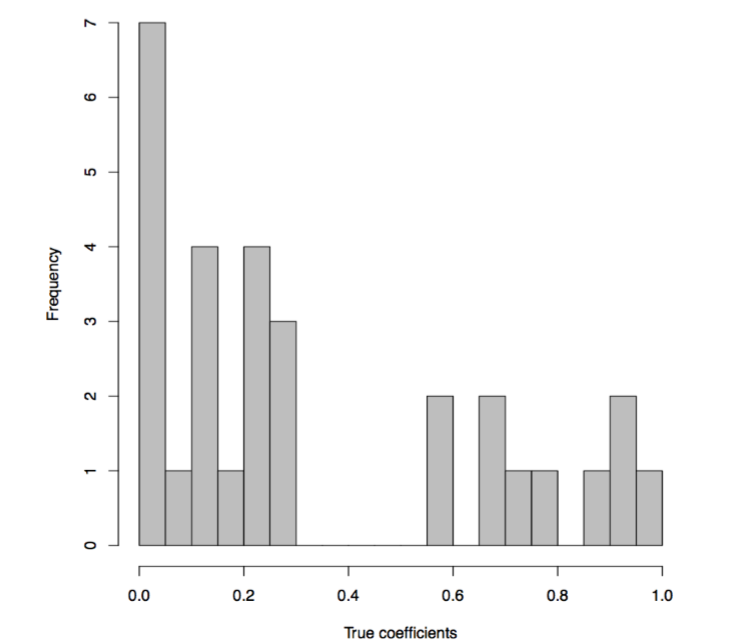
\includegraphics[scale = 0.4]{Test-Histogram}
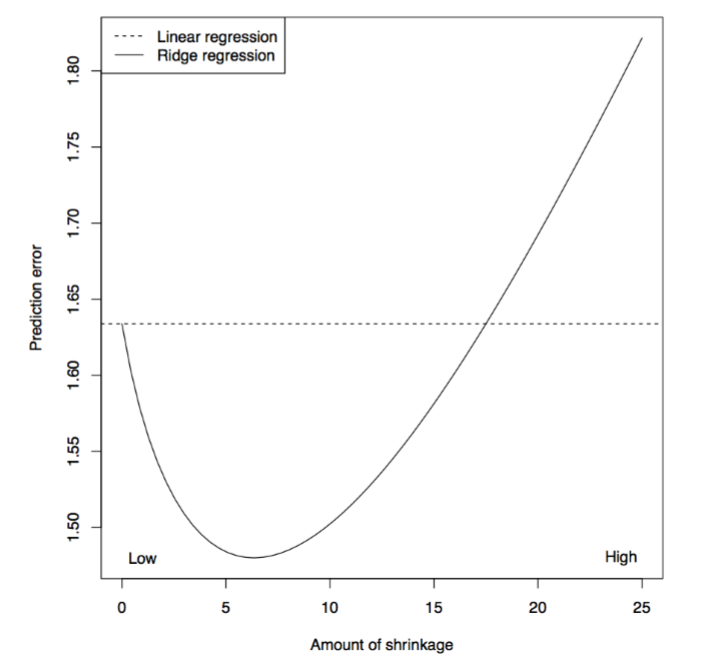
\includegraphics[scale = 0.4]{Shrink-to-Predict}
\\ \\
It is quite clear that there is a proper amount of shrinkage($\lambda$) such that the prediction error is at its minimum. The goal of ridge regression is to use that shrinkage for better prediction values. However, the shrinkage creates bias. As $\lambda$ increases, variance decreases while bias increases. 

\subsection{LASSO}
LASSO follows very similarly to ridge regression, however, LASSO actually shrinks coefficients to zero due to the $L_1$ norm of $\beta$. 

\begin{align}\nonumber
\hat{\beta}^{LASSO} &= arg\min_{\beta \in \mathbb{R}^p} RSS + \lambda\sum_{j=1}^p|\beta_j|\\\nonumber
&= \sum_{i=1}^n(y_i - x_i^T\beta)^2 + \lambda\sum_{j=1}^p|\beta_j| \\ 
&= ||y - X\beta||_2^2 + \lambda||\beta||_1
\end{align}
Similar to ridge regression, the following also apply to LASSO:
\begin{itemize}
\item $\lambda = 0$ results in no shrinkage
\item $\lambda \rightarrow \infty$ results in $\hat{\beta}^{ridge}$ going to zero 
\item $\lambda$ increases, variance decreases, bias increases
\end{itemize}
Since LASSO can shrink some coefficients to zero, it can be selective with the variables used in the model. As the shrinkage increases, more variables become zero, which result in the remaining variables shrinking even more. Both ridge and LASSO are effective shrinking methods that can be used for a wide variety of data. Due to the way they handle coefficient shrinking, ridge works better with more predictors with small true coefficients, while LASSO works better with less predictors and higher true coefficients as there will be less "overshrinkage" from zeroing out variables. 
\end{document}
